% -----------------------------------------------
% Template for ISMIR Papers
% 2016 version, based on previous ISMIR templates

% Requirements :
% * 6+1 page length maximum
% * 2MB maximum file size
% * Copyright note must appear in the bottom left corner of first page
% (see conference website for additional details)
% -----------------------------------------------

\documentclass{article}
\usepackage{ismir,amsmath,cite}
\usepackage{graphicx}
\usepackage{dsfont}
\usepackage{url}
\usepackage{color}

\usepackage{epstopdf} % convert eps to pdf

\usepackage{amsfonts}
\usepackage{stmaryrd}
\usepackage{xspace}
\usepackage{IEEEtrantools}
\newcommand*{\eg}{e.g.\@\xspace}
\newcommand*{\ie}{i.e.\@\xspace}
\newcommand*{\etal}{et al.\@\xspace}

% Title.
% ------
\title{Wavelet Scattering for Automatic Chord Estimation}

% Note: Please do NOT use \thanks or a \footnote in any of the author markup

% Single address
% To use with only one author or several with the same address
% ---------------
%\oneauthor
% {Names should be omitted for double-blind reviewing}
% {Affiliations should be omitted for double-blind reviewing}

% Two addresses
% --------------
%\twoauthors
%  {First author} {School \\ Department}
%  {Second author} {Company \\ Address}

%% To make customize author list in Creative Common license, uncomment and customize the next line
%  \def\authorname{First Author, Second Author} 


% Three addresses
% --------------
\threeauthors
 {First Author} {Affiliation1 \\ {\tt author1@ismir.edu}}
  {Second Author} {\bf Retain these fake authors in\\\bf submission to preserve the formatting}
  {Third Author} {Affiliation3 \\ {\tt author3@ismir.edu}}

%% To make customize author list in Creative Common license, uncomment and customize the next line
%  \def\authorname{First Author, Second Author, Third Author} 

% Four or more addresses
% OR alternative format for large number of co-authors
% ------------
%\multauthor
%{First author$^1$ \hspace{1cm} Second author$^1$ \hspace{1cm} Third author$^2$} { \bfseries{Fourth author$^3$ \hspace{1cm} Fifth author$^2$ \hspace{1cm} Sixth author$^1$}\\
%  $^1$ Department of Computer Science, University , Country\\
%$^2$ International Laboratories, City, Country\\
%$^3$  Company, Address\\
%{\tt\small CorrespondenceAuthor@ismir.edu, PossibleOtherAuthor@ismir.edu}
%}
%\def\authorname{First author, Second author, Third author, Fourth author, Fifth author, Sixth author}


\sloppy % please retain sloppy command for improved formatting

\begin{document}

%
\maketitle
%
\begin{abstract}
State-of-the-art automatic chord recognition systems rely on multi-band chroma representations,
Gaussian Mixture Model pattern matching, and Viterbi decoding.
This paper explores the use of Haar wavelet transforms and scattering in place of multi-band
chroma. Wavelets operating across octaves encode sums and differences in chroma bins at
different scales.
We describe both the Haar wavelet transform and deep wavelet scattering and develop an
efficient algorithm for their computation. Potential benefits of wavelet representations,
including stability to octave deformations, over multi-band chroma are discussed.
Accuracy of wavelet representations used for chord recognition is analyzed over a large
vocabulary of chord qualities.
\end{abstract}

%%%%%%%%%%%%%%%%%%%%%%%%%%%%%%%%%%%%%%%%%%%%%%%%%%

\section{Introduction}\label{sec:introduction}
Along with lyrics and melody, chord sequences provide a succinct description of tonal music.
As such, they are often written down under the form of lead sheets, for the use of
accompanists and improvisers.
Besides its original purpose in music education and transmission, the knowledge of
harmonic content has been leveraged in music information research to address higher-level
tasks, including cover song identification \cite{ellis2007identifying},
genre recognition \cite{perez2009genre}, and lyrics-to-audio alignment
\cite{mauch2012integrating}. We refer to the review of McVicar \etal
\cite{mcvicar2014automatic} for a recent state of the art.

As stressed by Humphrey and Bello \cite{humphrey2015four}, chord labels
are not mutually exclusive categories, but instead follow a relation of partial order.
For instance, the tetrad \texttt{A:min7} is contained in the triad
\texttt{A:min}, which in turn is contained in the power chord \texttt{A:5}.
By setting up equivalence rules for chord labels that belong to a common
superset, discrepancies between conflicting annotations can be resolved
up to a desired level of specificity.
In spite of this variety of settings, all evaluation metrics for automatic
chord estimation share the following minimal property:
a chord label remains the same if all its components are jointly
transposed by one octave, be it upwards or downwards.

In order to comply with this requirement, the vast majority of existing
systems rely on the chroma representation, \ie a 12-dimensional vector
derived from the constant-Q spectrum by summing up all
frequency bands which share the same pitch class, according to
the twelve-tone equal temperament.
However, it should be noted that the chroma representation is not
only invariant to octave transposition, but also to any permutation
of the chord factors -- an operation known in music theory
as inversion.
Yet, although major and minor triads are unchanged by inversion,
some rarer chords, such as augmented triads and minor seventh
tetrads, are conditional upon the position of the root.

Figure 1 illustrates the importance of disambiguating inversions
when transcribing chords. The first two voicings are identical up
to octave transposition of all the chord factors, and thus have the
same chord label $\texttt{A:min7}$.
In contrast, the third voicing is labeled as \texttt{C:maj6}
in root position, although its third inversion would correspond
to the first voicing.

\begin{figure}[t]
    \begin{center}
        \setlength{\unitlength}{1cm}
        \begin{picture}(8.5,1.5)
        \put(0,-0.5){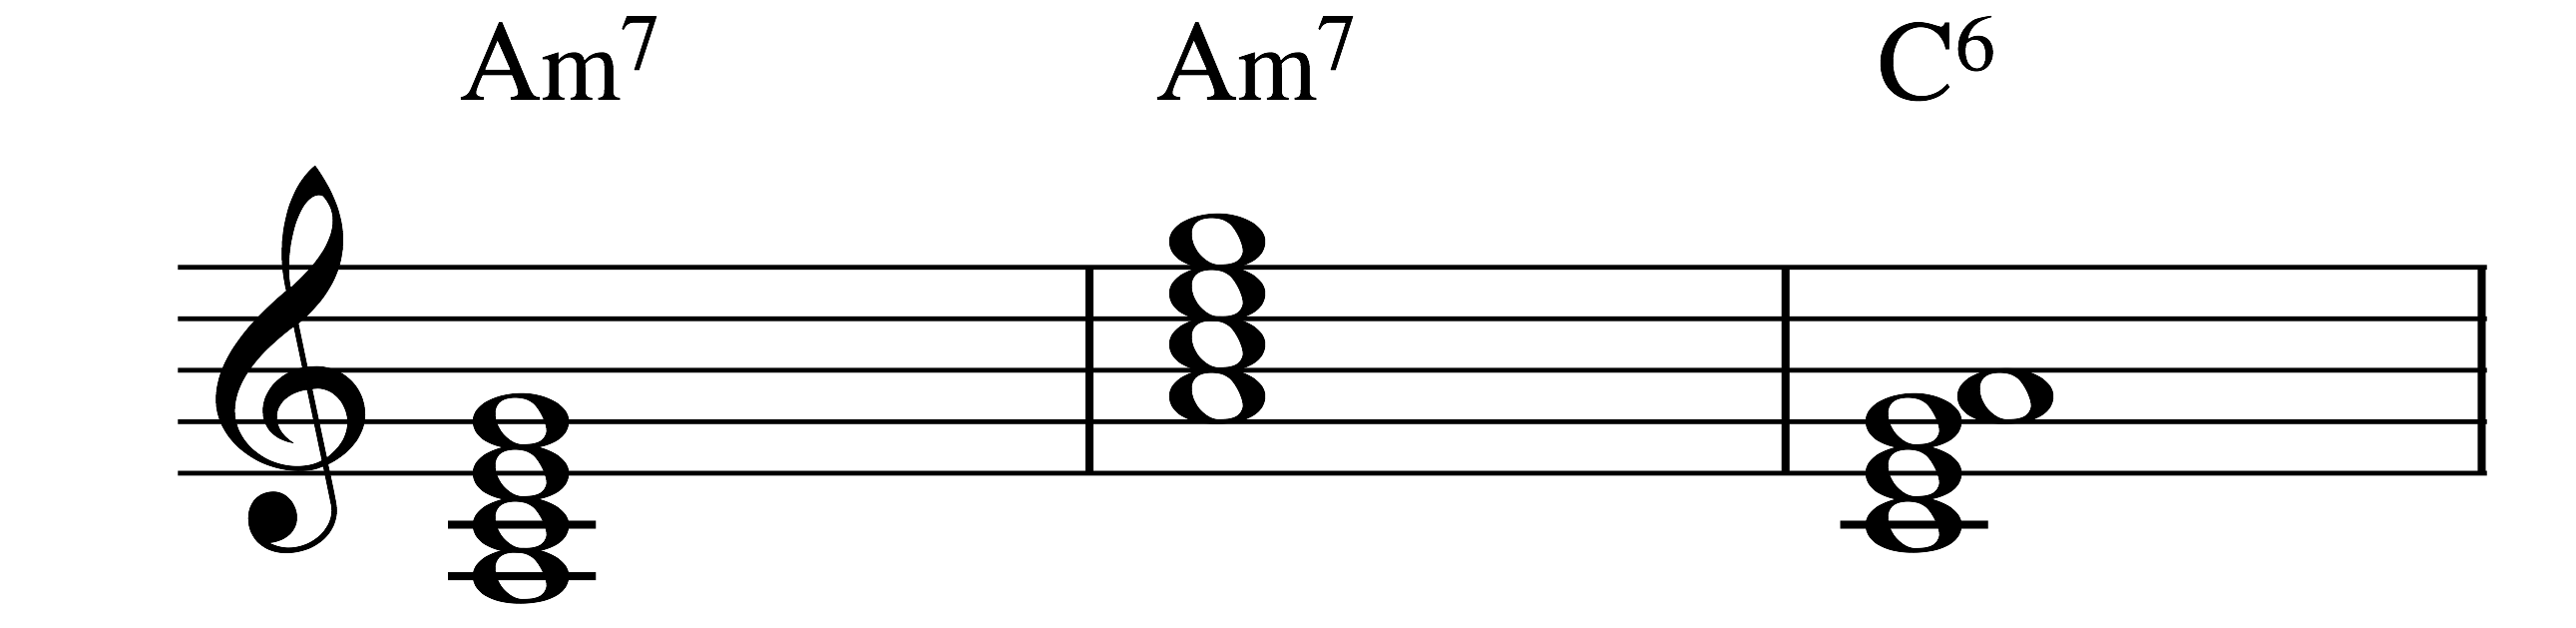
\includegraphics[width=8.5cm]{figs/sheet_music.png}}
        \end{picture}
    \end{center}
    \protect\caption{
Three possible voicings of the pitch class set
$\texttt{\{C,E,G,A\}}$, resulting either in the chord \texttt{A:min7}
or \texttt{C:maj6}. See text for details.
\label{fig:sheet-music}
}
\end{figure}

With the aim of improving automatic chord estimation under fine-grained
evaluation metrics, this article introduces two feature extraction methods
that are invariant to octave transposition, yet sensitive to
chord inversion.
The former consists in computing Haar wavelet transform of
the constant-Q spectrum along the octave variable and keeping
the absolute values of the resulting coefficients, at all scales
and positions.
The latter iterates the Haar wavelet modulus nonlinear operator
over increasing scales, until reaching the full extent of the
constant-Q spectrum.
Both methods build upon the software of Cho and Bello
\cite{cho2013mirex}, which holds state-of-the-art performance on
the McGill Billboard dataset \cite{burgoyne2011}.

Section 2 describes the multi-band chroma features, as
introduced by Cho and Bello, and its integration into a multi-stream
hidden Markov model.
Section 3 defines the Haar wavelet transform across octaves
of the constant-Q spectrum.
Section 4 defines the deep Haar scattering transform.
Section 5 discusses the efficiency of the presented systems over
a dataset of 65 Beatles songs, according to different evaluation
metrics and parameter settings.

\section{Multi-band chroma features}
A system for automatic chord estimation typically consists of two stages:
feature extraction and acoustic modeling.
At the first stage, the audio query is converted into a time series of
pitch class profiles, which represent the relative salience of
pitch classes according to the twelve-tone equal temperament.
At the second stage, each frame in the time series is assigned
a chord label among a predefined vocabulary.
This section presents a multi-stream approach to acoustic modeling,
as first introduced by Cho and Bello \cite{cho2013mirex}.

The constant-Q transform $\boldsymbol{X}[t, \gamma]$ is a time-frequency
representation whose center frequencies $2^{\gamma/Q}$ are in a geometric progression.
By setting $Q=12$, the log-frequency variable $\gamma$ is akin to a pitch in twelve-tone
equal temperament.
Moreover, the Euclidean division $\gamma = Q \times j + u$
reveals the octave $u$ and pitch class $q$,
which play an essential role in music harmony.
In all of the following, we reshape the constant-Q transform
accordingly, and keep the notation $\boldsymbol{X}[t, q, u]$ for simplicity.

Let us recall that the chroma representation consists in summing up
octaves $u$ at fixed time $t$ and pitch class $q$:
\begin{equation}
\boldsymbol{Y}[t, q]
= 
\sum_{u} \boldsymbol{X}[t, q, u].
\end{equation}

To address the disambiguation of chords in an extended vocabulary,
Cho and Bello have divided the constant-Q spectrum into $K$
bands, by means of half-overlapping Gaussian windows along
the log-frequency axis \cite{cho2013mirex}.
The width $\sigma$ of the windows is inversely proportional
to the desired number of bands $K$:
it is of the order of one octave for $K=8$,
and two octaves for $K=4$.
The centers of the windows are denoted by $\gamma_k$, where
the band index $k$ ranges from $0$ to $K-1$.
Consequently, the multi-band chroma features are defined as the following
three-way tensor:
\begin{equation}
\boldsymbol{Y}[t, q, k]
=
\sum_{u} 
\boldsymbol{X}[t, q, u]
\boldsymbol{w}[Q \times j + u - \gamma_k],
\end{equation}
where
$\boldsymbol{w}[\gamma] = \exp( - \gamma^2 / (2\sigma^2))$
is a Gaussian window of width $\sigma$, centered around zero.

Because some chord transitions are more frequent than others,
acoustic modeling is classically achieved with a hidden Markov model (HMM)
whose states are estimated as mixtures of multivariate Gaussian probability
distributions, \ie Gaussian mixture models (GMM), in dimension $Q=12$.
In order to extend this framework to multi-band chroma features, Cho and Bello
have trained $K$ models in parallel, end-to-end, over each band $k$
of the tensor $\boldsymbol{Y}[t, q, k]$.
At test time, the emission probability distributions of each model
are aggregated such that they are the predicted outputs of a single state sequence.

The computational complexity of resulting $K$-stream HMM grows exponentially
with the number of streams $K$.
However, by assuming synchronicity and statistical independence of the streams,
the aggregation boils down to a geometric mean, thus with linear complexity in $K$.
It must be noted that the geometric mean does not yield a true probability distribution, as
it does not sum to one.
Yet, it is of widespread use in speech recognition, due to its simplicity and computational
tractability.

%%%%%%%%%%%%%%%%%%%%%%%%%%%%%%%%%%%%%%%%%%%%%%%%%%

\section{Haar Wavelet Transform}\label{sec:haar}
Dating back to 1909, the Haar wavelet $\psi$ is a piecewise constant, real function of compact
support, consisting of two steps of equal length and opposite values. Within a discrete framework,
it is defined by the following formula:
\begin{equation}
\forall u \in \mathbb{Z}, \;
\boldsymbol{\psi}[u] = \left\{ \begin{array}{cl}
\frac{-1}{\sqrt{2}} & \mbox{if }u = 0\\
\frac{1}{\sqrt{2}} & \mbox{if }u = 1\\
0 & \mbox{otherwise}
\end{array}\right.
\end{equation}
The "mother" wavelet $\boldsymbol{\psi}[u]$ is translated and dilated by powers of two, so as to
produce a family of discrete sequences
$\boldsymbol{\psi_{j,b}}[u] = 2^{j/2} \boldsymbol{\psi}[2^j (u - 2b)]$
indexed by the scale parameter $j \in \mathbb{N}$ and the translation parameter $b \in \mathbb{Z}$.
After endowing them with the Euclidean inner product
\begin{equation}
\langle \boldsymbol{\psi_{j,b}} \vert \boldsymbol{\psi_{j^\prime,b^\prime}} \rangle
 =
 \sum_{u = -\infty}^{+\infty}
 \boldsymbol{\psi_{j, b}}[u]
  \boldsymbol{\psi_{j^\prime,b^\prime}}[u],
\end{equation}
the wavelets $\{\boldsymbol{\psi_{j,b}}\}_{j,b}$ form an orthonormal basis of finite-energy
real sequences.
Moreover, the Haar wavelet is the shortest function of compact support such that the family
$\{\boldsymbol{\psi_{j,b}}\}_{j,b}$ satisfies this orthonormality property.
On the flip side, it has a poor localization in the Fourier domain, owing to its sharp discontinuities.

It must be noted that, unlike the pseudo-continuous variables of time and frequency,
the octave variable is intrinsically dicrete, and has no more than 8 coefficients in
the audible spectrum.
As such, we choose to favor compact support over regularity, \ie Haar over
Daubechies or Gabor wavelets.
Elements of the Haar wavelet basis are shown on Figure \ref{fig:haar-wavelets}
for various values of $j$ and $b$.

\begin{figure}[t]
    \begin{center}
        \setlength{\unitlength}{1cm}
        \begin{picture}(8.5,8.8)
        \put(0,-0.5){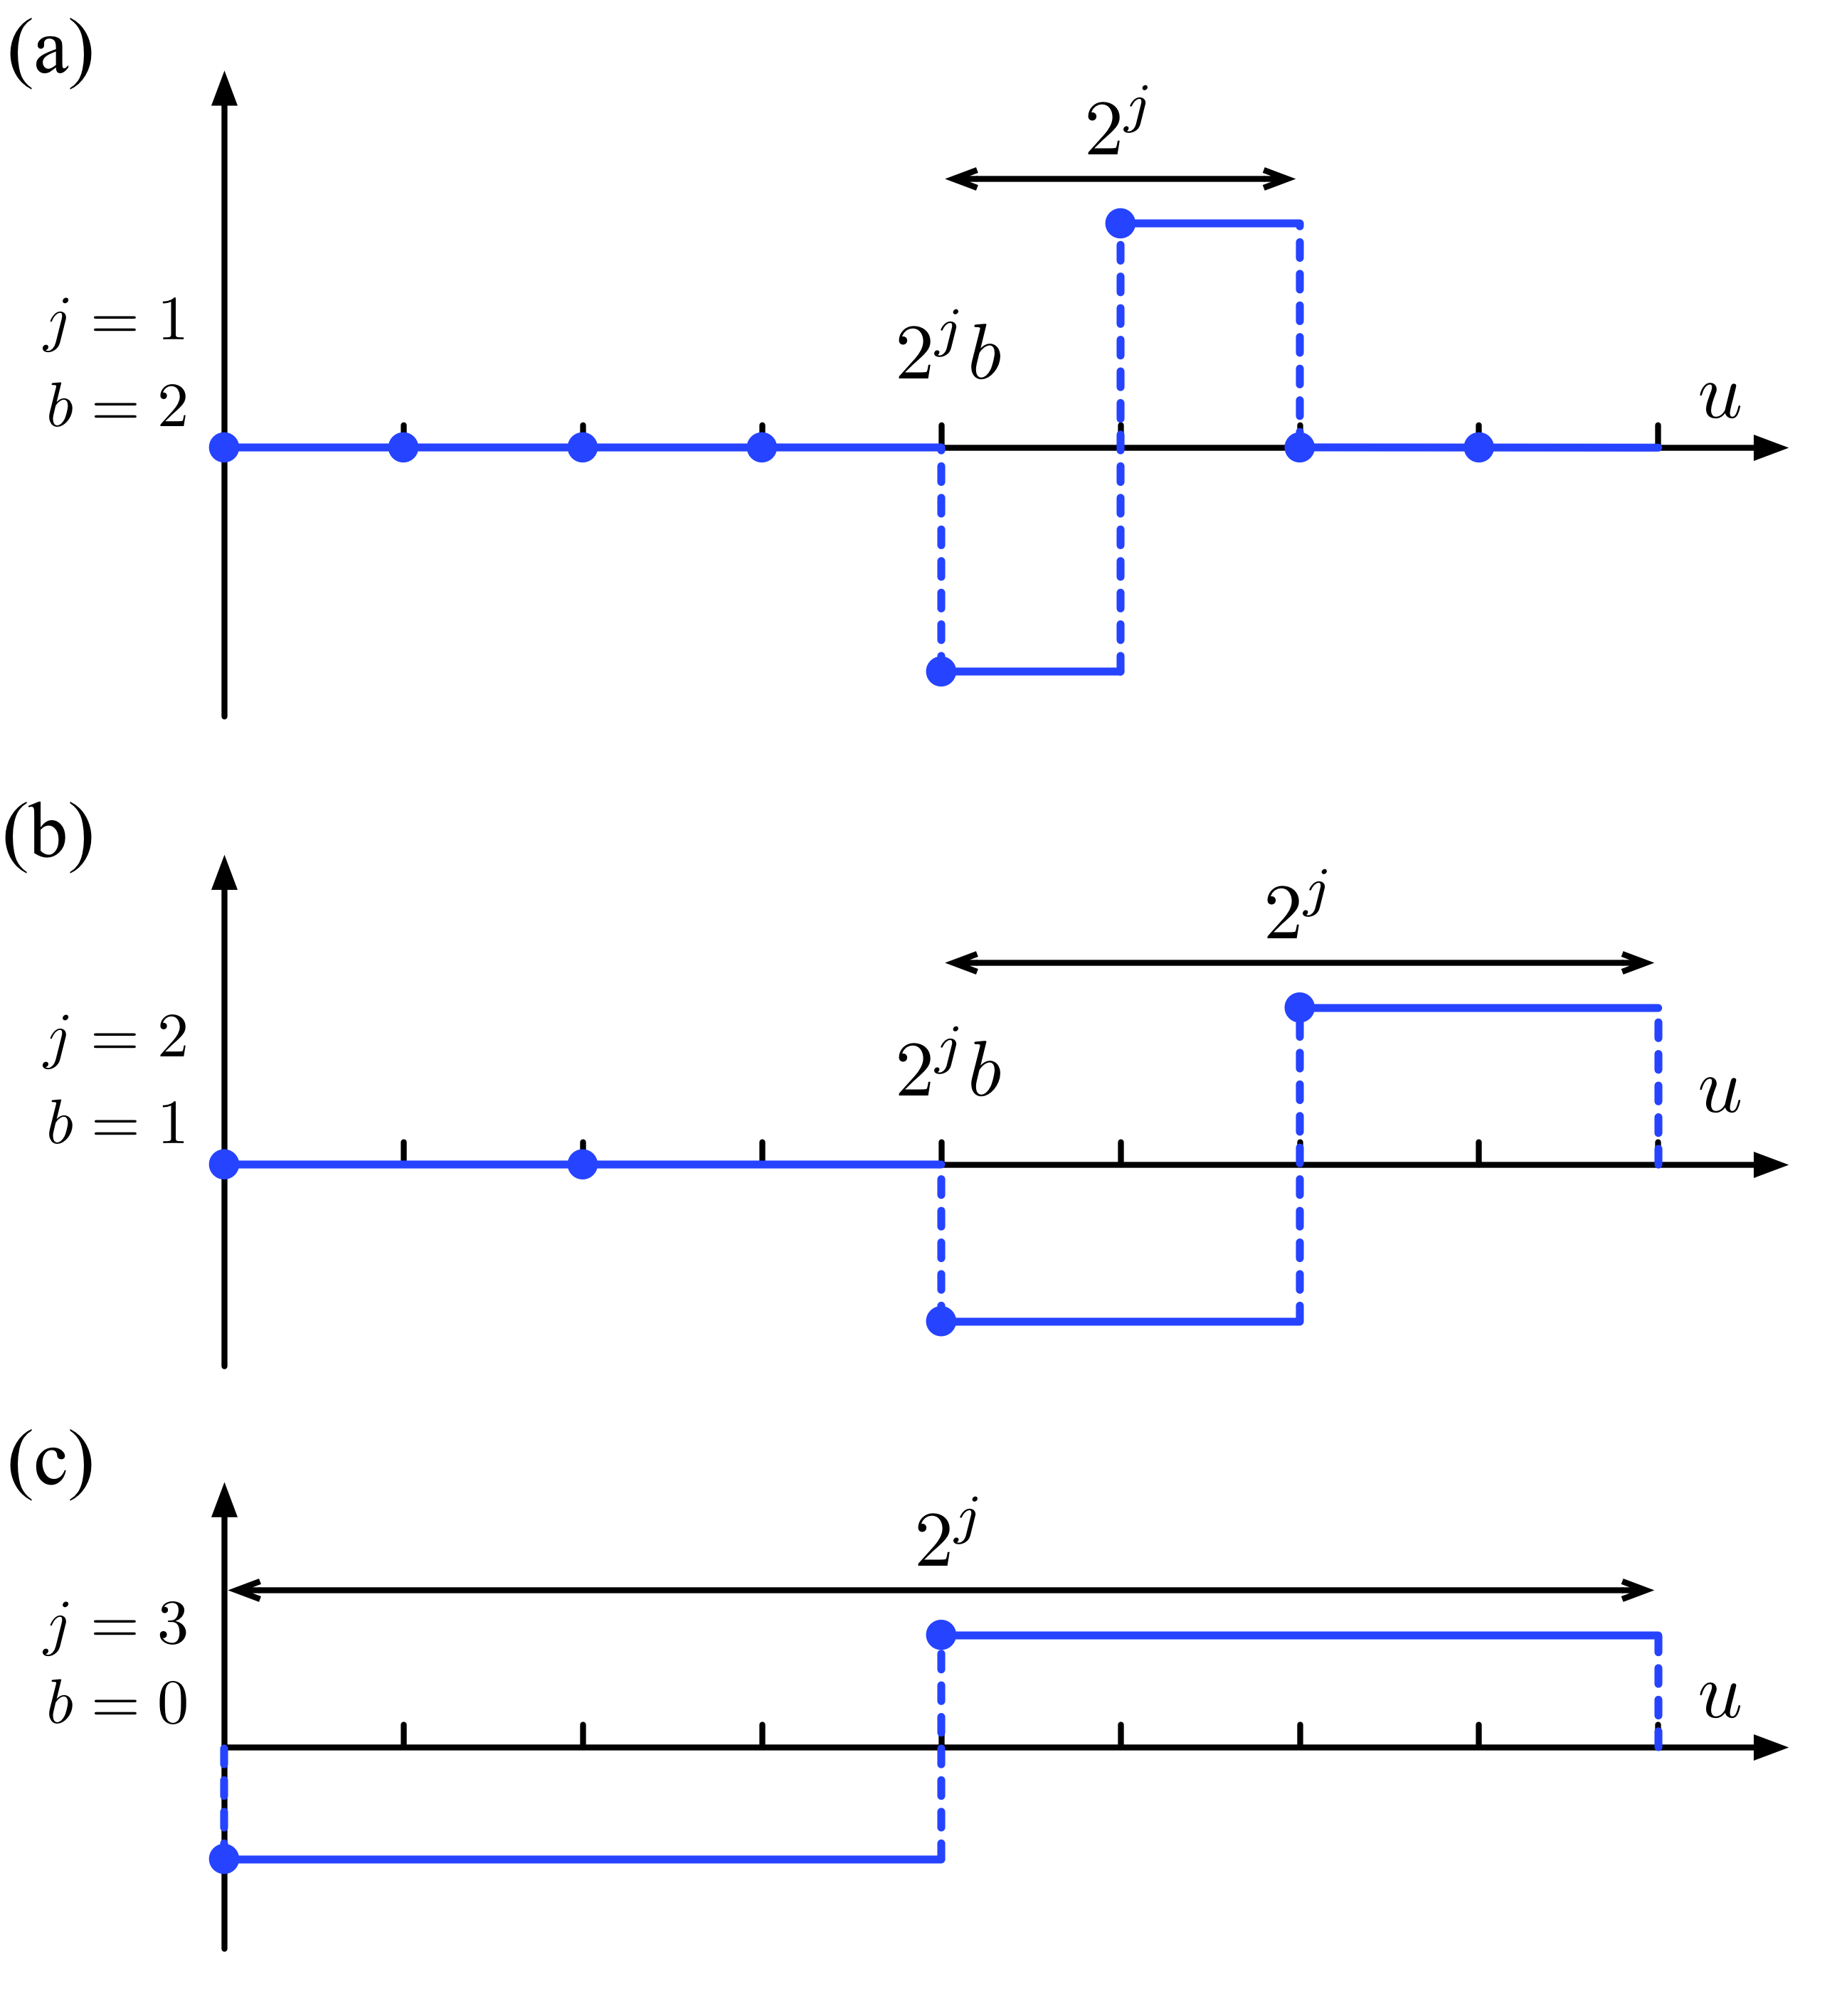
\includegraphics[width=8.5cm]{figs/haar_functions.png}}
        \end{picture}
    \end{center}
    \protect\caption{
Three elements of the Haar wavelet basis $\{ \boldsymbol{\psi_{j,b}}\}$
for various values of the scale index $j$ and the translation index $b$.
See text for details.
\label{fig:haar-wavelets}
}
\end{figure}

The wavelet transform coefficients of some finite-energy sequence
$\boldsymbol{x} \in \ell^2(\mathbb{Z})$ are defined by
$\boldsymbol{Wx}[j, b] = \langle \boldsymbol{x} \vert \boldsymbol{\psi_{j,b}} \rangle$.
Since $\boldsymbol{x}[u]$ has a finite length $K = 2^J$, the above decomposition is informative
only for indices $(j, b)$ such that $j < J$ and $2^j b < K$, that is $b<2^{J-j}$.
The number of coefficients in the Haar wavelet transform of $\boldsymbol{x}[u]$ is thus equal to
$\sum_{j<J} 2^{J-j} = 2^J - 1$. For the wavelet representation to
preserve energy and allow signal reconstruction, a residual term
\begin{equation}
\boldsymbol{A_J x}
= \boldsymbol{x}[0] -
\sum_{j,b}
\langle \boldsymbol{x} \vert \boldsymbol{\psi_{j,b}} \rangle \boldsymbol{\psi_{j,b}}[0]
= \sum_{u<K} \boldsymbol{x}[u]
\end{equation}
must be appended to the wavelet coefficients.
Observe that $\boldsymbol{A_J x}$ computes a delocalized average of all signal
coefficients, which can equivalently be formulated as an inner product with the constant
function $\boldsymbol{\phi}[u] = 2^{-J/2}$ over the support $\llbracket 0 ; K \llbracket$.
Henceforth, it corresponds to the traditional chroma representation, where spectrogram bands
of the same pitch class $q$ are summed across all $K$ octaves.

Since the wavelet representation amounts to $K$ inner products in $\mathbb{R}^K$,
its computational complexity is $\Theta(K^2)$ if implemented as a matrix-vector product.
Implementing these inner products as convolutions would bring the complexity to
$\Theta{(K (\log_2 K)^2)}$ by using the Fast Fourier Transform (FFT) algorithm.
To improve this, Mallat has developed a recursive scheme, called
\emph{multiresolution pyramid} \cite{mallat1989theory}, which operates as a cascade
of convolutions with some pair of quadrature mirror filters
$(\boldsymbol{g}, \boldsymbol{h})$ and progressive downsamplings by a factor of two.

\begin{equation}
\boldsymbol{Wx}[j,b] =
\left(
\boldsymbol{h_{\downarrow 2}} \circ
\boldsymbol{g_{\downarrow 2}} \circ \ldots \circ
\boldsymbol{g_{\downarrow 2}}\boldsymbol{x}
\right)[b]
\end{equation}

\begin{equation}
\boldsymbol{A_J x} =
\boldsymbol{g_{\downarrow 2}} \circ \ldots \circ
\boldsymbol{g_{\downarrow 2}}\boldsymbol{x}
\end{equation}

The associated Z-transforms $G$ and $H$ of $\boldsymbol{g}$
and $\boldsymbol{h}$ satisfy the quadrature mirror property $G(z) = H(-z)$ and
energy conservation: $\vert G(z) \vert ^2 + \vert H(z) \vert ^2 = 1$.
The interested reader can refer to chapter 7 of Mallat's textbook \cite{mallat2008wavelet},
of which we adopt the mathematical notations.

In the case of Haar wavelets, the low-pass filtering $(\boldsymbol{x} \ast \boldsymbol{g})$
consists of the sum between adjacent coefficients, whereas the high-pass filtering
$(\boldsymbol{x} \ast \boldsymbol{h})$ is the coresponding difference, up to a
renormalization constant:

\begin{equation}
(\boldsymbol{x}
\ast
\boldsymbol{g})[2b]
=
\frac{ \boldsymbol{x}[2b+1] + \boldsymbol{x}[2b]}{\sqrt{2}}
=
\boldsymbol{x}[2b]
-
\langle \boldsymbol{x} \vert \boldsymbol{\psi_{0,b}} \rangle
\end{equation}

\begin{equation}
(\boldsymbol{x}
\ast
\boldsymbol{h})[2b]
=
\frac{ \boldsymbol{x}[2b+1] - \boldsymbol{x}[2b]}{\sqrt{2}}
=
\langle \boldsymbol{x} \vert \boldsymbol{\psi_{0,b}} \rangle.
\end{equation}

\begin{figure}[t]
    \begin{center}
        \setlength{\unitlength}{1cm}
        \begin{picture}(8,2.5)
        \put(0,-0.5){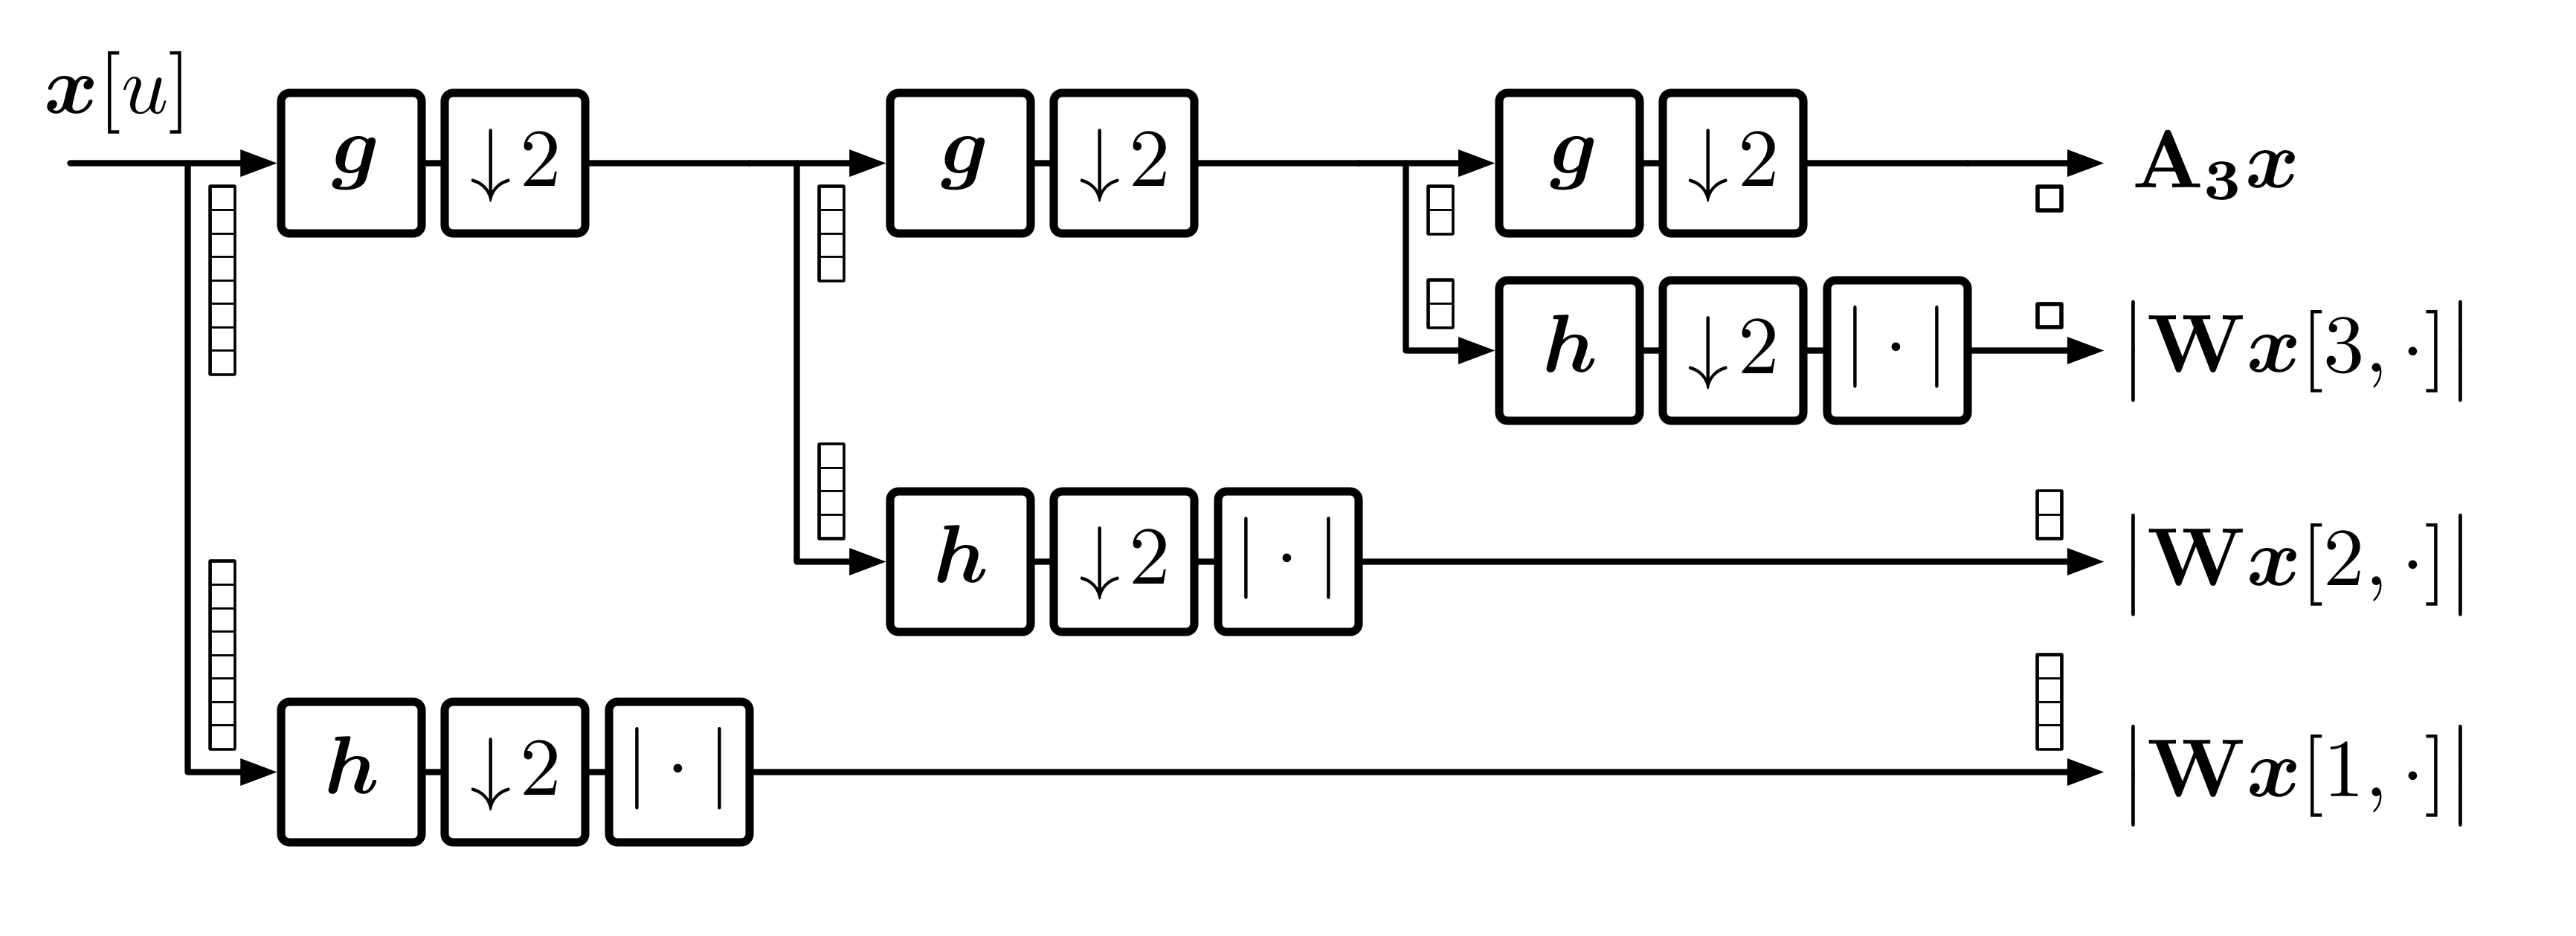
\includegraphics[width=7cm]{figs/wavelet_scheme.png}}
        \end{picture}
    \end{center}
    \protect\caption{
    Discrete wavelet transform of a signal of length 8, as implemented with a
    convolutional pyramid scheme. See text for details.
\label{fig:haar-wavelets}
}
\end{figure}

\begin{table}
	\begin{center}
	\begin{tabular}{|c|cc|}
		\hline
		& operations & memory \\
		\hline
		Matrix-vector product & $\Theta(K^2)$ & $\Theta(K)$ \\
		Fast Fourier transform & $\Theta(K (\log K)^2)$ & $\Theta(K)$ \\
		Multiresolution pyramid & $\Theta(K \log K)$ & $\Theta(1)$ \\
		\hline		
	\end{tabular}
	\end{center}
	\caption{
	Computational complexity and memory usage of various implementations
	of the Haar wavelet transform, for a one-dimensional signal of length $K$.
	See text for details.
	\label{table:wavelet-complexities}}
\end{table}


%%%%%%%%%%%%%%%%%%%%%%%%%%%%%%%%%%%%%%%%%%%%%%%%%%

\section{Deep Haar Scattering}\label{sec:scattering}

% don't forget to cite sifre when writing about fast deep scattering
% Explain the organization of scattering paths along the vertices of a binary cube.
Two neighboring samples $\boldsymbol{x}[2b]$ and $\boldsymbol{x}[2b+1]$ can
be retrieved, up to a permutation, from the absolute values of the subsampled QMF
decomposition $(\boldsymbol{g_{\downarrow 2}x}, \boldsymbol{h_{\downarrow 2}x})$:
\begin{equation}
\max_{u\in\{2b, 2b+1\}} \boldsymbol{x}[u] =
\dfrac{\vert \boldsymbol{g_{\downarrow 2}x}\vert [b]+
\vert \boldsymbol{h_{\downarrow 2}x}\vert [b]}{\sqrt{2}}
\end{equation}

\begin{equation}
\min_{u\in\{2b, 2b+1\}} \boldsymbol{x}[u] =
\dfrac{
\vert \boldsymbol{g_{\downarrow 2}x} \vert [b] - 
\vert \boldsymbol{h_{\downarrow 2}x} \vert [b]}{\sqrt{2}}
\end{equation}

	As opposed to the Haar wavelet transform representation, a Haar scattering representation concatenates sum and difference terms at different scales and then iterates. From the chroma representation $\chi_{t,q,z}$, we reshape to a tensor of dimension $J+2$ called $\phi$:
	
	\begin {equation}
	\chi_{t,q,z} \rightarrow \phi_{t,q,\sigma_1, \sigma_2, \ldots , \sigma_J}
	\end{equation}
	
	where the size of $\phi$ is $T \times Q \times 2_1 \times 2_2 \ldots \times 2_J$. At each scale $j \in [1, J]$, we first create a copy of $\phi$ called $\hat{\phi}$, and then concatenate the sum of $\hat{\phi}$ along scale $\sigma_j$ and the difference of $\hat{\phi}$ along $\sigma_j$, setting the result as $\phi$. We then take the modulus $| \phi | $ and iterate. 
	
\begin{figure}[t]
    \begin{center}
        \setlength{\unitlength}{1cm}
        \begin{picture}(8,7)
        \put(0.1,0){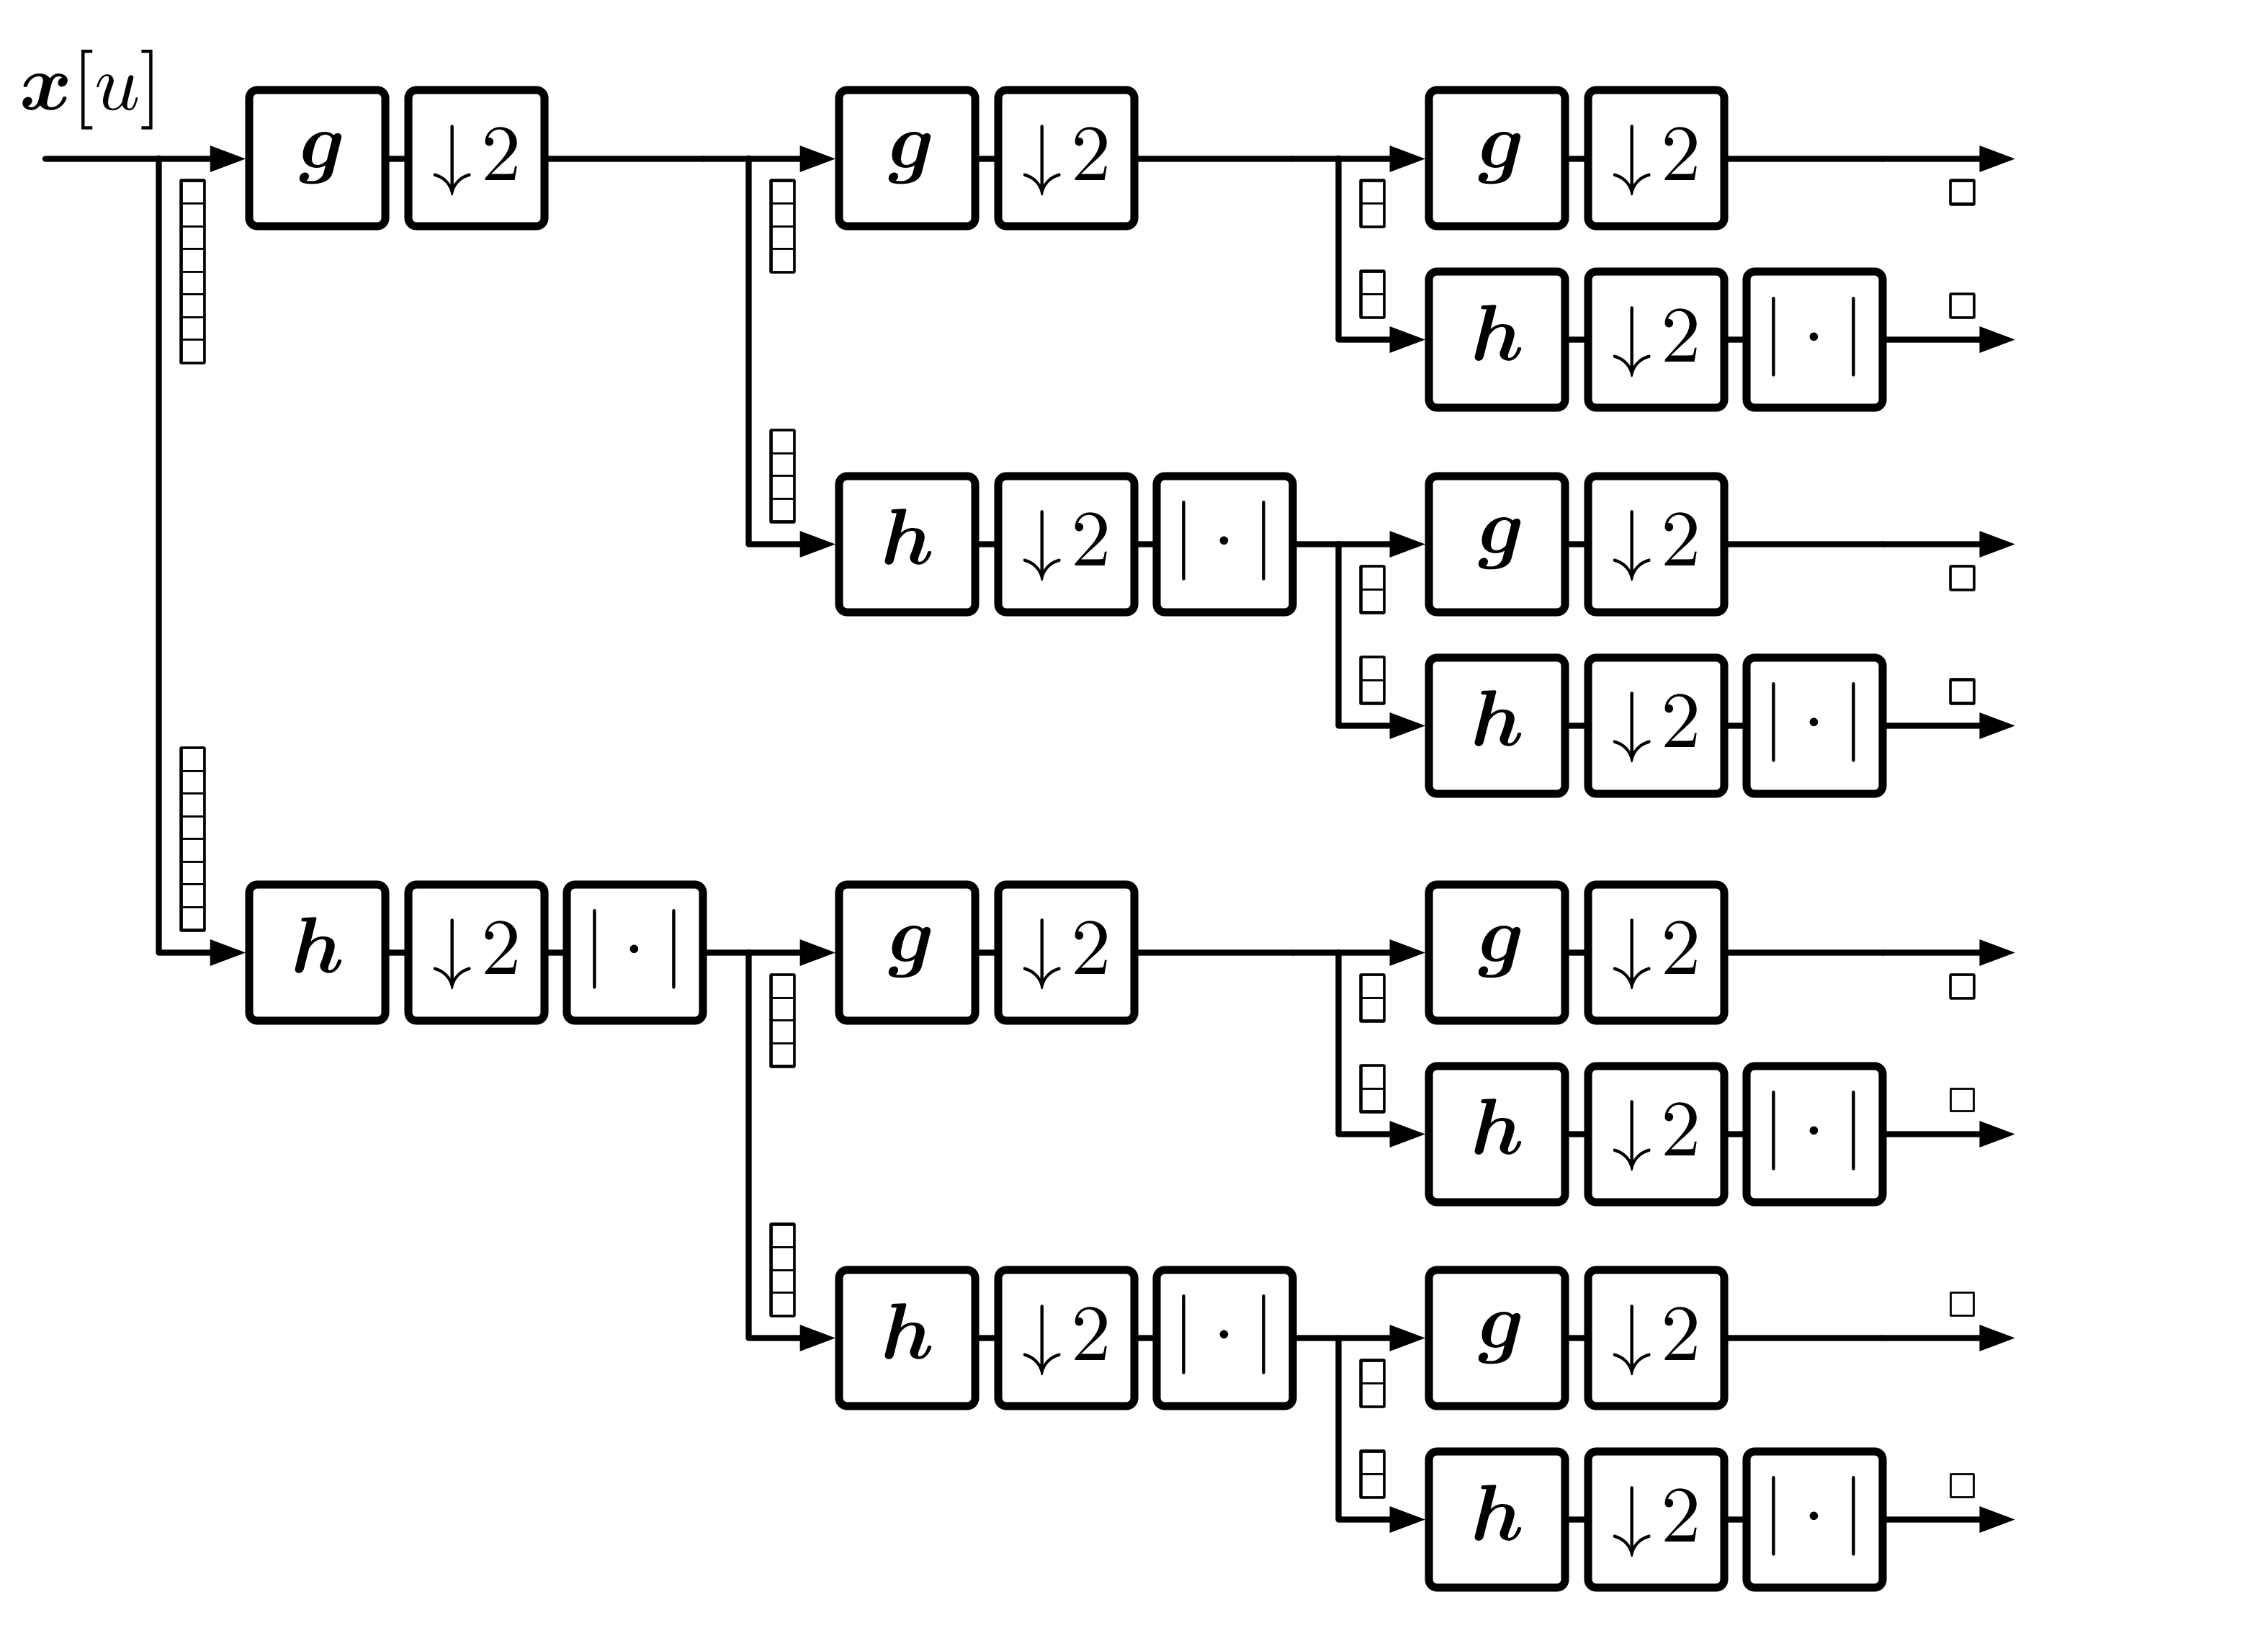
\includegraphics[width=8cm]{figs/scattering_scheme.png}}
        \end{picture}
    \end{center}
    \protect\caption{
    Deep scattering transform of a signal of length 8, as implemented with a convolutional
    pyramid scheme. See text for details.
\label{fig:haar-scattering}
}
\end{figure}

\begin{table}
	\begin{center}
	\begin{tabular}{|c|cc|}
		\hline
		& operations & memory \\
		\hline
		Matrix-vector product & $\Theta(K^3)$ & $\Theta(K^2)$ \\
		Fast Fourier transform & $\Theta(K^2 (\log K)^2)$ & $\Theta(K^2)$ \\
		Multiresolution pyramid & $\Theta(K^2 \log K)$ & $\Theta(1)$ \\
		\hline		
	\end{tabular}
	\end{center}
	\caption{Computational complexity and memory usage of various implementations
	of the deep Haar scattering transform, for a one-dimensional signal
	of length $K$. See text for details.
	\label{table:scattering-complexities}}
\end{table}


%%%%%%%%%%%%%%%%%%%%%%%%%%%%%%%%%%%%%%%%%%%%%%%%%%
\section{Experimental Setup and Evaluation}\label{sec:experiment}
	
% What are those 157 chords ? Explain 13 x 12 + 1
\textbf{Pattern matching} is done by creating a chord model for all 157 chords with Gaussian Mixture
Models (GMMs). This is a supervised learning approach where features are extracted
for a large training set that contains examples of all 157 chords (with annotations) and are
then used to train GMM templates for each chord. Data augmentation is employed by rotating each
chord through the chroma space so that one example of C minor can also train a model for
C\# minor, D minor, etc. For any temporal frame $t$, each of the $K$ chroma representations
$\boldsymbol{Y}_{t,q,k}$ are matched using GMMs and then fused together via geometric mean.
Finally, \textbf{decoding} uses Hidden Markov Model (HMM) systems to post-filter the pattern
matched data.

Here, we use the Viterbi algorithm, which describes the transition probability from
one chord $C_i$ state to another -- $\mathds{P}(C_i \rightarrow C_j)$, therefore filtering out chord
transitions that are highly unlikely. The matrix of transition probabilities for Viterbi decoding is
generated from the labeled training data.

Evaluation of an ACE system was determined using some of the tools found in the
mir\_eval library \cite{raffel2014mir} and written into a simple python script which compared the
estimated chords coming out of the ACE system to the ground truth annotations for all songs
in the testing set.
All experiments were run on the High Performance Computing (HPC) environment at
NYU's Courant Institute. 
	
For each experiment, a chord model and Viterbi transition probability matrix are generated from a 
training set of 451 songs.
The 'band' ($K$) of any experiment determines the amount of chroma vectors at any given temporal
window -- equivalent to the number of bands in the multiband chroma representation, and the
maximum wavelet scale in the wavelet and scattering representations (\ie the number of wavelet
coefficients). Chord recognition is then carried out on the testing set of 65 songs.
Both the training set and testing set of songs are kept constant across all experiments.
	
After generating estimated chord labels for each song in the test set,
a Python script evaluates the results.
As per \cite{raffel2014mir}, there is ``no single right way to compare two sequences of chord labels,"
and the mir\_eval package computes ACE accuracy based along metrics such as root, triads,
maj/min, sevenths, inversions, etc.
For simplicity, we evaluate all experiments using the mirex measure, which ``considers a chord
correct if it shares at least three pitch classes in common" \cite{raffel2014mir}.
	
State of the art systems such as those in \cite{cho2014on} use a multiband chroma feature
extraction with $K = 4$ windowed bands.
To begin, some baseline trials were run on a training set consisting of 108 songs from the Beatles
discography, 99 RWC pop songs, 224 songs from the Billboard dataset, and 20 Queen songs,
for a total of 451 songs.
Our testing dataset comprised of 65 songs from the Beatles and uspop datasets that were not part
of the training set and that contained a sufficient number of examples of each chord quality. 
		
The constant-Q spectrogram $\boldsymbol{X}[t, \gamma]$ is reshaped into a time-chroma-octave
representation $\boldsymbol{X}[t, q, u]$ where the chroma index $q \in \llbracket 0 ; Q \llbracket$ and
octave index $u \in \llbracket 0 ; K \llbracket$ are derived from the log-frequency index $\gamma$
by Euclidean division: $\gamma = Q \times u + q$.
All subsequent operations apply to the octave variable $u$, and are vectorized in terms of time
$t$ and chroma $u$. To alleviate notations, we replace the three-way tensor $\boldsymbol{X}[t, q, u]$
by a vector $\boldsymbol{x}[u]$, thus leaving the indices $t$ and $q$ implicit.


When applied to the chroma representation $\boldsymbol{X}(t,q,z)$, where $t$ is a temporal window, $q$ a chroma pitch class (an integer between 1 and 12), and $z$ an octave, the Haar wavelet transform encodes the sums and differences in chroma bins across octaves.
The number of output ``bands" from the Haar wavelet transform, given by $k$, determines the number of scales $J$ for which the basis Haar wavelet is dilated: $2^J = k$.

The use of the Haar wavelet transform in the feature extraction stage for our ACE system is motivated by the fact that it is stable to octave deformations -- something that the multiband representation is not. By coding for chroma relationships across varying octave scales, we are able to capture representations at both low scales (less invariance, more stability) and higher scales (higher invariance, less stability), thereby reducing the variance of the GMMs. 
	
	The Haar wavelet transform is then computed iteratively over the scale $J  = log_2(k)$ and stored into a cell of size $k$, with each row in the cell containing a chroma matrix of size $T \times Q$ (same as in the multiband case, but with $k=8$ cell rows instead of 4). At each scale $j \in \llbracket1, J\rrbracket$, the chroma tensor $\boldsymbol{X}[t,q,z]$ is reshaped to a four dimensional tensor $g$ from which the sum $g$ and difference $h$ coefficients are calculated:
	
	\begin{equation}
	\boldsymbol{X}[t,q,z] \rightarrow g[t,q,w,v]
	\end{equation}
	
	where
	
	\begin{equation}
	\mathrm{size}(\boldsymbol{X}) = (T \times Q \times Z) \hspace{0.3cm} \rightarrow \hspace{0.3cm}  \mathrm{size}(g) = (T \times Q \times 2 \times \frac{k}{2^j})
	\end{equation}
	
	$h$ takes the difference of $g$ along the third dimension ($\partial g/\partial w = h$). For each $v \in [1, \frac{k}{2^j}]$, the modulus $| h_{t,q,w,v}|$ is stored as a row in the output Haar wavelet representation cell. $g$ is then summed along the third dimension ($w$) and squeezed down into a three dimensional tensor (singleton dimensions due to sum removed). After iterating at all scales, the resulting $g$ is stored as the last ($k$'th) row in the output Haar cell array.
		
%%%%%%%%%%%%%%%%%%%%%%%%%%%%%%%%%%%%%%%%%%%%%%%%%%

\section{Results}\label{sec:results}

\begin{figure}
 \centerline{
 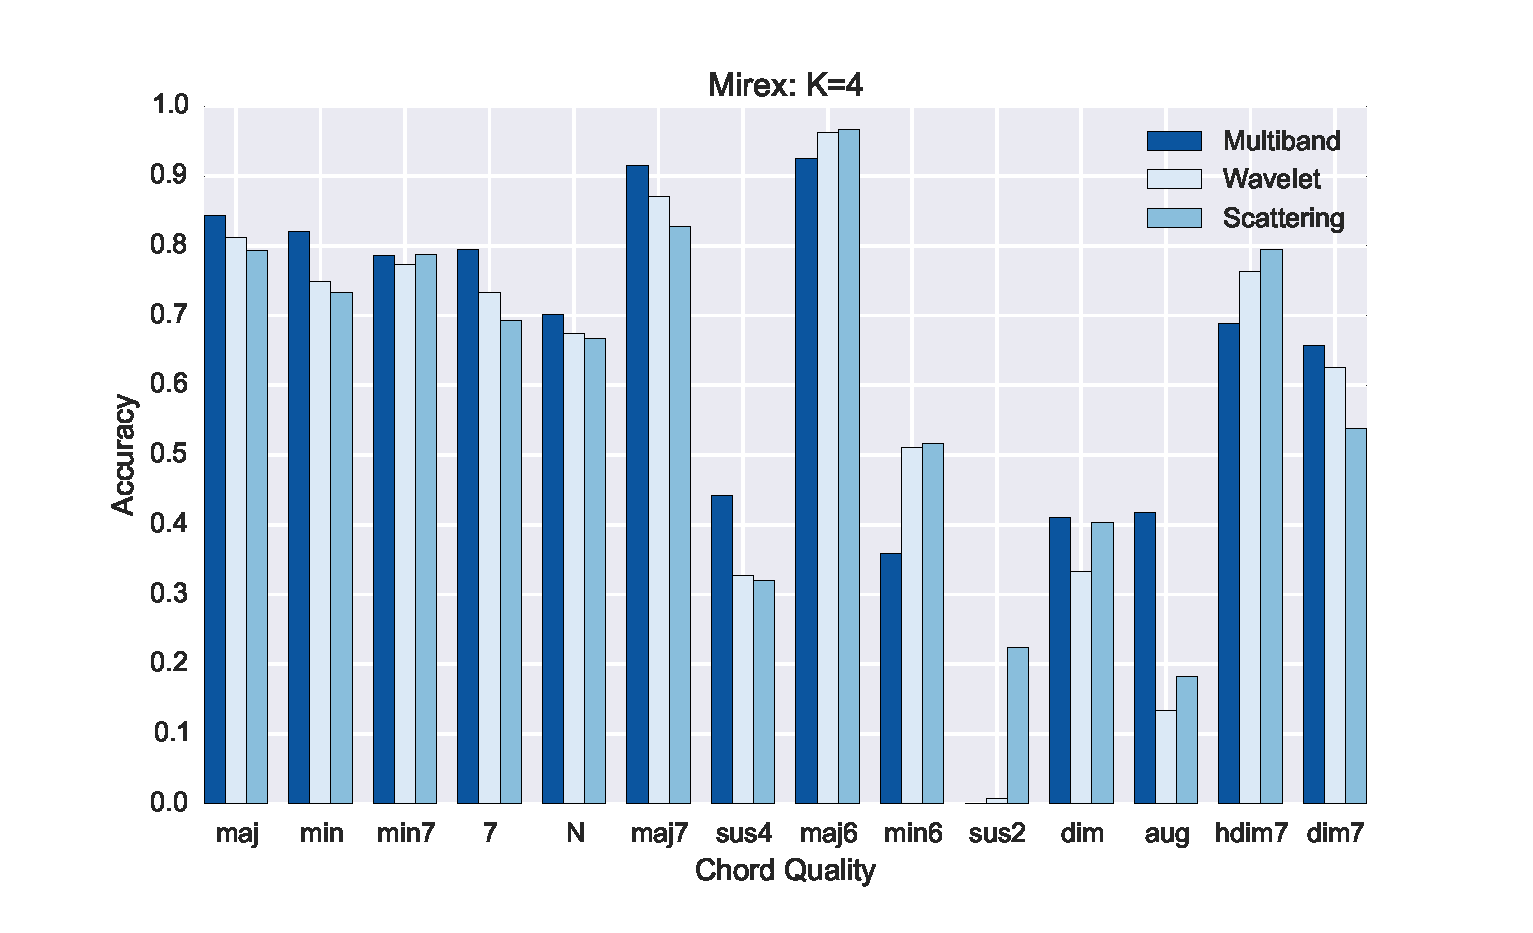
\includegraphics[width=10cm]{figs/mirex4.eps}}
 \caption{Multiband (chroma), Haar wavelet transform, and deep Haar scattering compared for $K=4$ streams. Chord accuracy computed via mirex.}
 \label{fig:mirex4}
\end{figure}

\begin{figure}
 \centerline{
 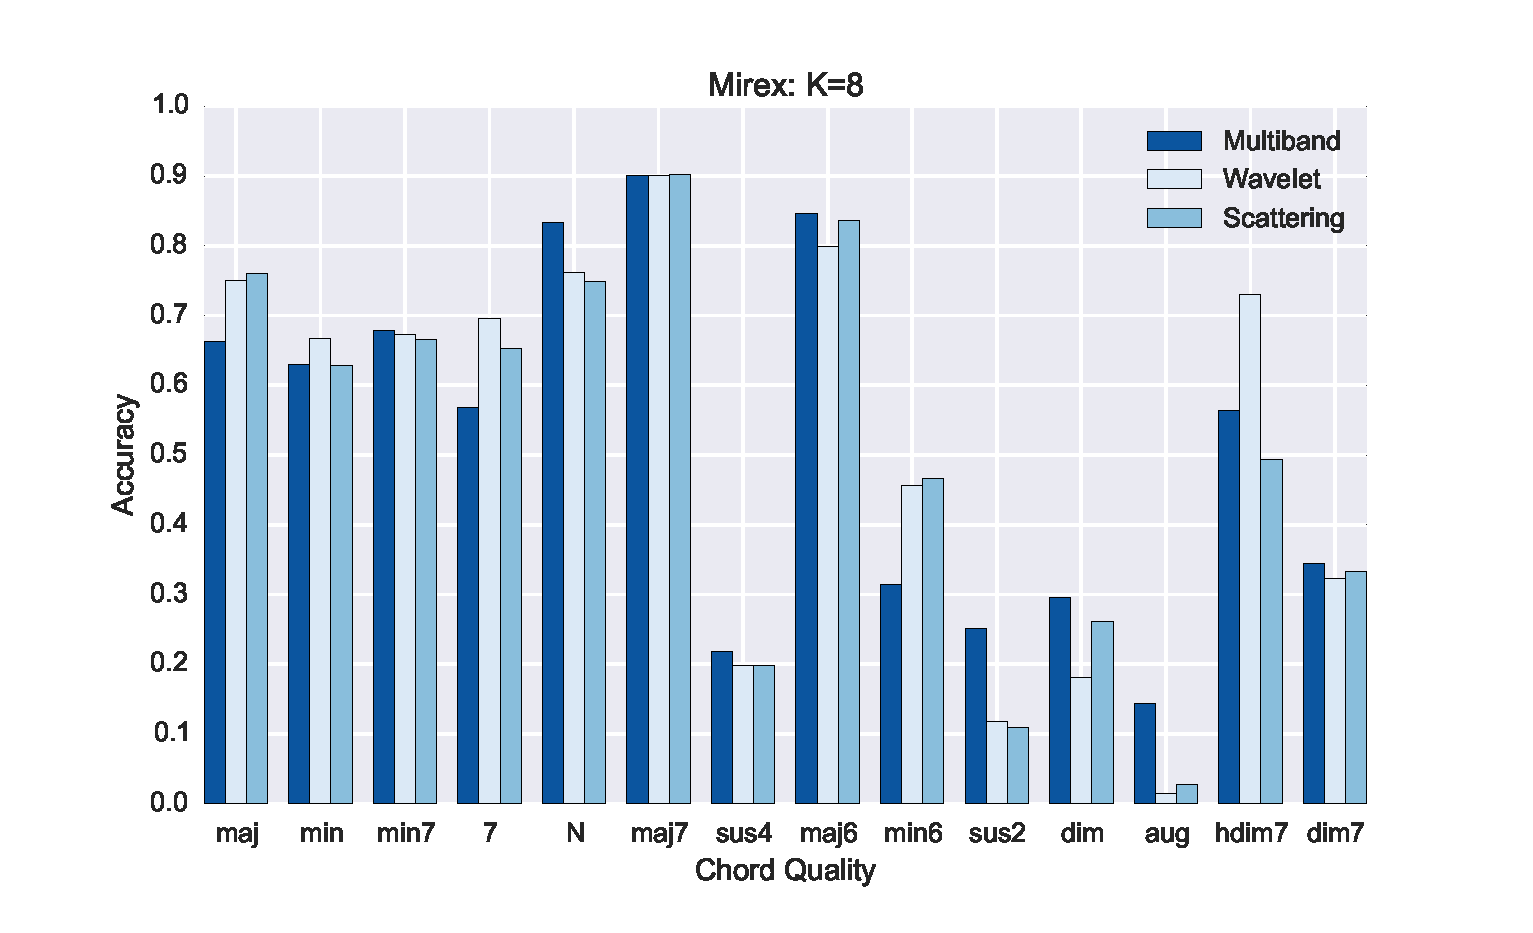
\includegraphics[width=10cm]{figs/mirex8.eps}}
 \caption{Multiband (chroma), Haar wavelet transform, and deep Haar scattering compared for $K=8$ streams. Chord accuracy computed via mirex.}
 \label{fig:mirex8}
\end{figure}


\begin{figure}
 \centerline{
 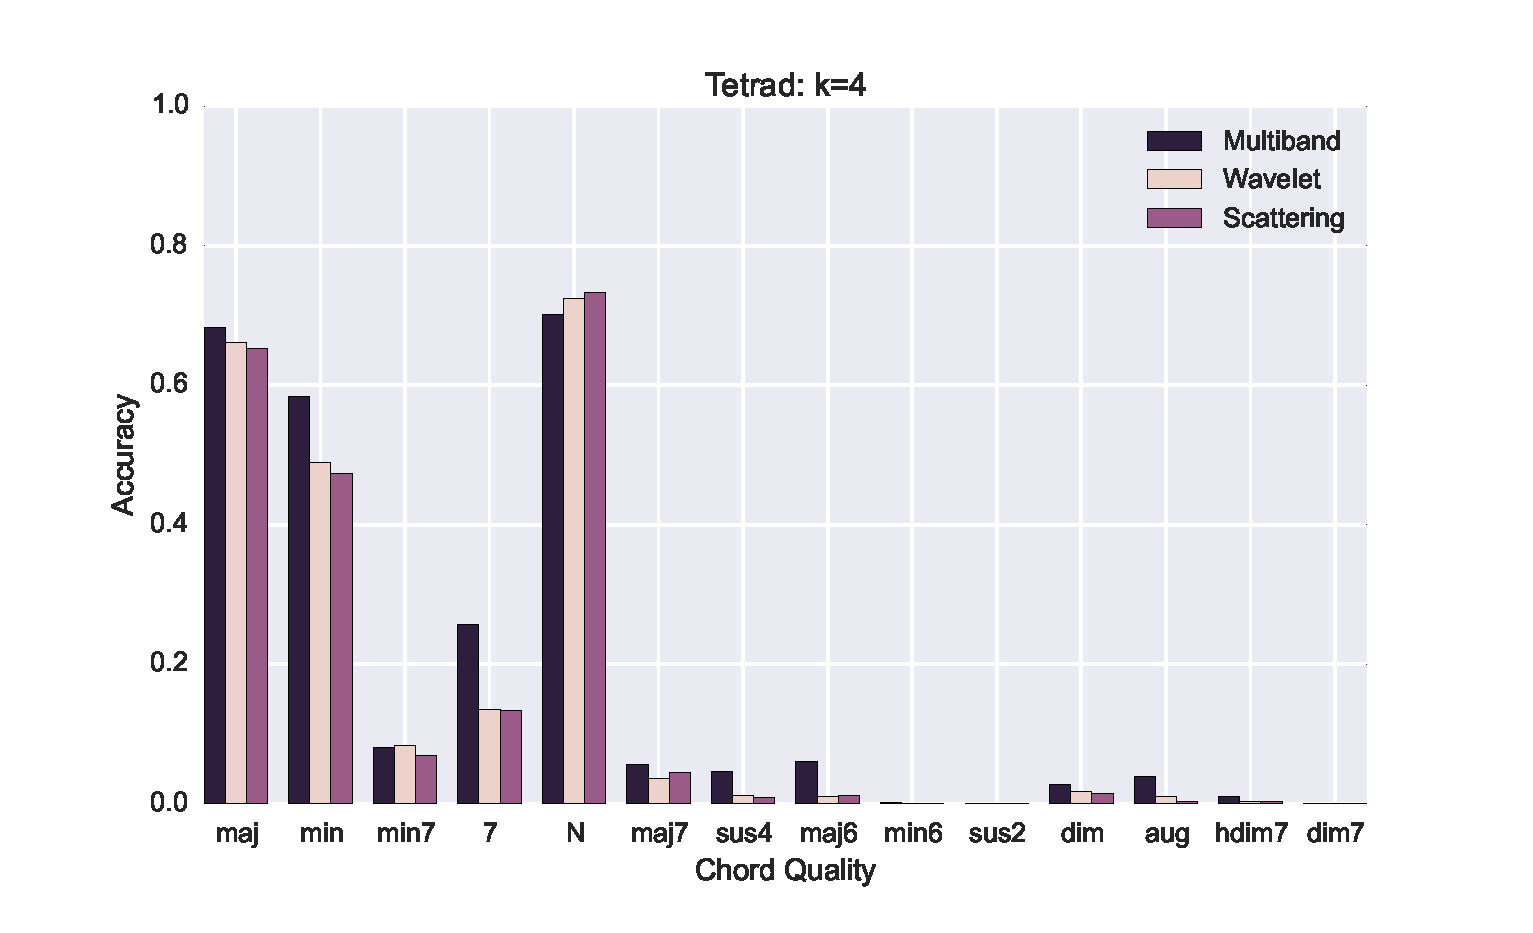
\includegraphics[width=10cm]{figs/tetrad4.eps}}
 \caption{Multiband (chroma), Haar wavelet transform, and deep Haar scattering compared for $K=4$ streams. Chord accuracy computed via tetrad.}
 \label{fig:tetrad4}
\end{figure}

\begin{figure}
 \centerline{
 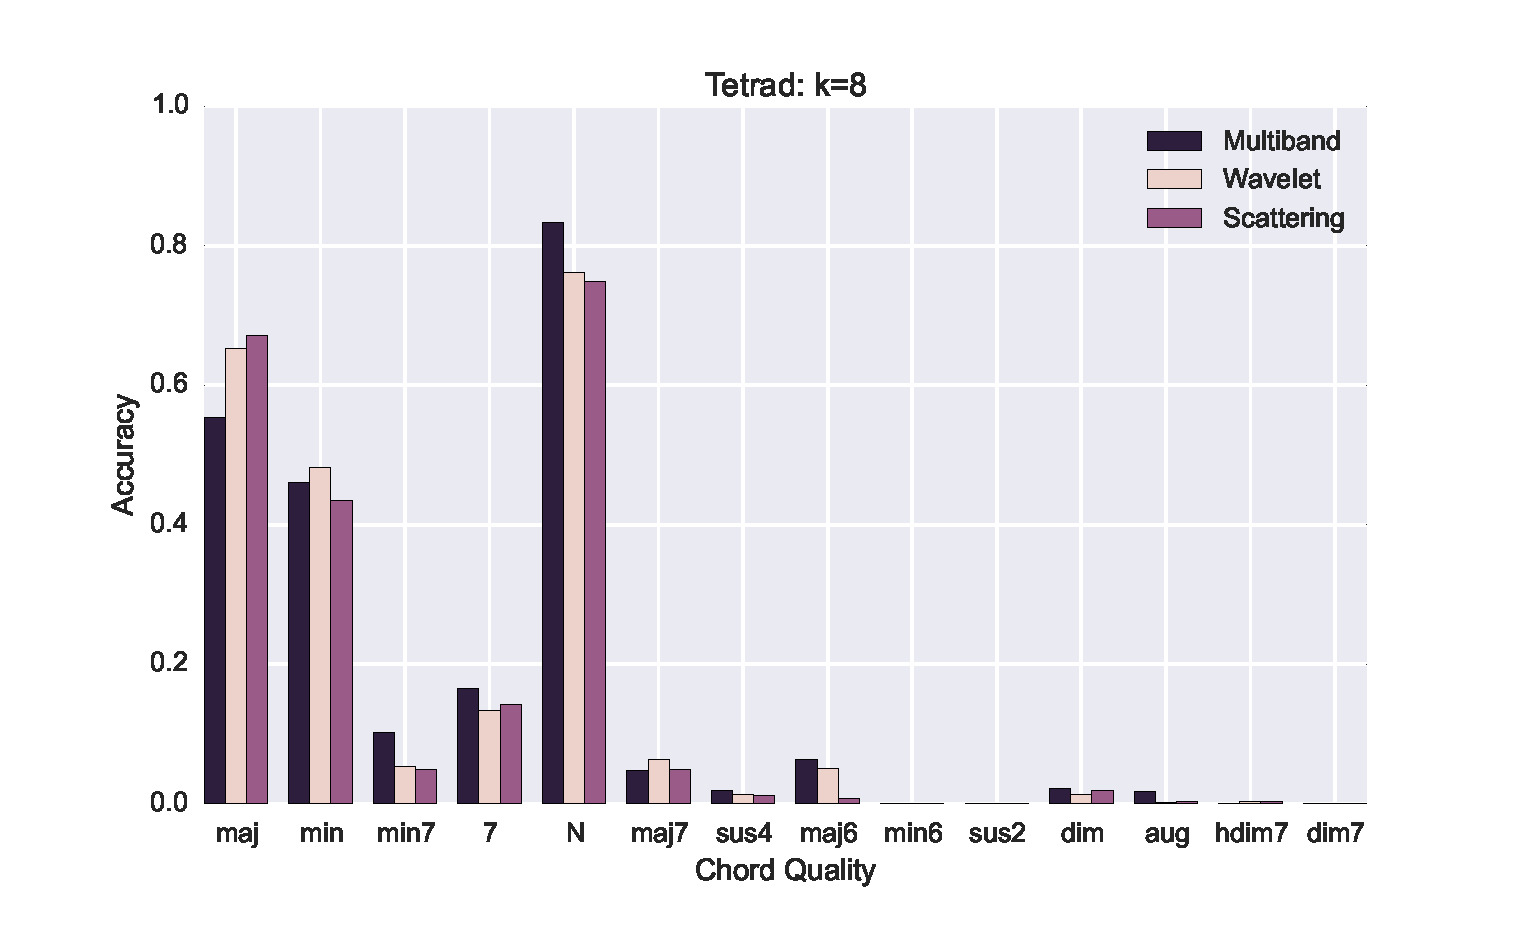
\includegraphics[width=10cm]{figs/tetrad8.eps}}
 \caption{Multiband (chroma), Haar wavelet transform, and deep Haar scattering compared for $K=8$ streams. Chord accuracy computed via tetrad.}
 \label{fig:tetrad8}
\end{figure}

~Results and discussion forthcoming.~
	
%%%%%%%%%%%%%%%%%%%%%%%%%%%%%%%%%%%%%%%%%%%%%%%%%%

\section{Discussion}\label{sec:discussion}

~Results and discussion forthcoming.~

%%%%%%%%%%%%%%%%%%%%%%%%%%%%%%%%%%%%%%%%%%%%%%%%%%

% For bibtex users:
\bibliography{WaveletScatteringISMIR2016}
\bibliographystyle{ieeetr}

% For non bibtex users:
%\begin{thebibliography}{citations}
%
%\bibitem {Author:00}
%E. Author.
%``The Title of the Conference Paper,''
%{\it Proceedings of the International Symposium
%on Music Information Retrieval}, pp.~000--111, 2000.
%
%\bibitem{Someone:10}
%A. Someone, B. Someone, and C. Someone.
%``The Title of the Journal Paper,''
%{\it Journal of New Music Research},
%Vol.~A, No.~B, pp.~111--222, 2010.
%
%\bibitem{Someone:04} X. Someone and Y. Someone. {\it Title of the Book},
%    Editorial Acme, Porto, 2012.
%
%\end{thebibliography}

\end{document}
